

Enclosing the CMS tracker and calorimeters is a \SI{3.8}{T} superconducting solenoid magnet---the most powerful in the world. The cylindrical structure of the solenoid measures \SI{6}{m} in internal diameter and \SI{12.5}{m} long, seen in the photograph in Fig.~\ref{fig:Magnet}. The high magnetic field inside the solenoid is necessary to induce sufficient bending of charged particle trajectories in the transverse plane so precise $p_T$ measurements can be made by the tracker. Outside the solenoid is a ferromagnetic return yoke made of construction steel, divided into five wheels w in the barrel region labeled YBw and three disks n in each (positive and negative) endcap labeled YE$\pm$n. The return yoke induces a strong magnetic field within the muon system (mounted to the return yoke) that improves the $p_T$ measurements of muons. The direction of the bending of particles inside the tracker and muon systems is also used to identify the charge sign. The solenoid magnet also serves as a support structure for the \SI{10000}{ton} steel return yoke.

\begin{figure}[H]
    \centering
    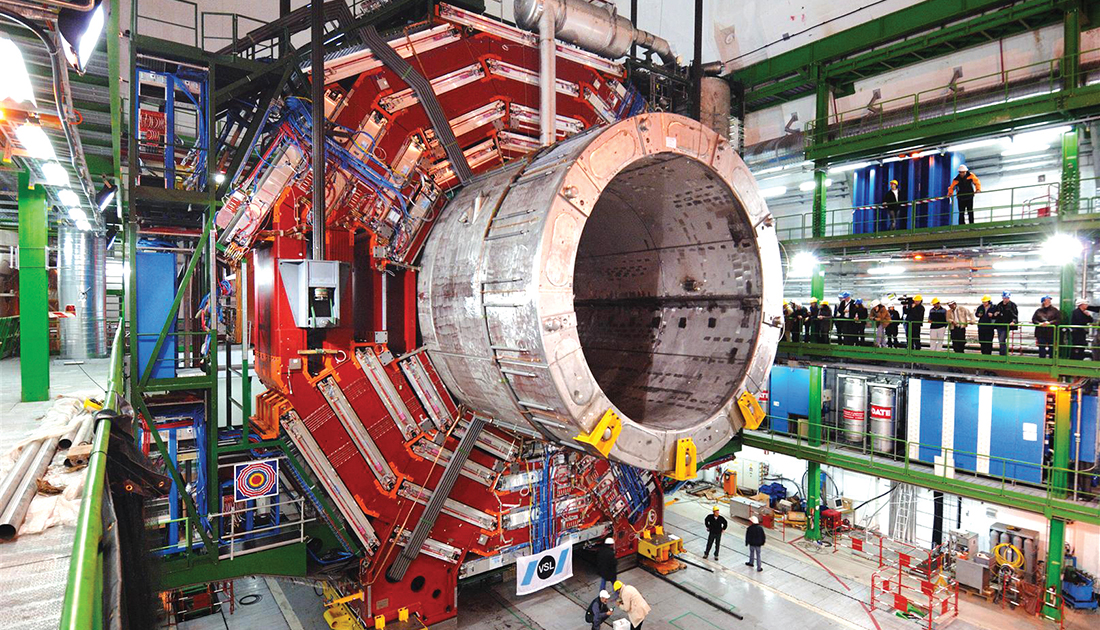
\includegraphics[width=\textwidth]{Images/CMS/Magnet.jpg}
    \caption{The solenoid magnet of CMS together with a wheel of the steel return yoke.}
    \label{fig:Magnet}
\end{figure}
